\documentclass[10pt,a4paper]{article}

\usepackage[utf8]{inputenc}
\usepackage[margin=1.2in]{geometry}
\usepackage[french]{babel}
\usepackage{amsmath}
\usepackage{amsfonts}
\usepackage{graphicx}
\usepackage{hyperref}
\usepackage[nottoc, notlof, notlot]{tocbibind}
\hypersetup{colorlinks=true,citecolor=black,filecolor=black,linkcolor=black,urlcolor=black}
\setlength{\parindent}{0.6cm} 
\setlength{\parskip}{0.10cm}
\usepackage[automark]{scrpage2}
\usepackage{color, colortbl}
\usepackage[table]{xcolor}

%% http://www.cnam.fr/maths/Membres/ghorbanzadeh/
\usepackage[T1]{fontenc}
\usepackage{listings}

%%configuration de listings
\lstset{
language=c++,
basicstyle=\ttfamily\small, %
identifierstyle=\color{red}, %
keywordstyle=\color{blue}, %
stringstyle=\color{black!60}, %
commentstyle=\it\color{green!95!yellow!1}, %
columns=flexible, %
tabsize=2, %
extendedchars=true, %
showspaces=false, %
showstringspaces=false, %
numbers=left, %
numberstyle=\tiny, %
breaklines=true, %
breakautoindent=true, %
captionpos=b
}

\usepackage{xcolor}

\definecolor{Zgris}{rgb}{0.87,0.85,0.85}

\newsavebox{\BBbox}
\newenvironment{DDbox}[1]{
\begin{lrbox}{\BBbox}\begin{minipage}{\linewidth}}
{\end{minipage}\end{lrbox}\noindent\colorbox{Zgris}{\usebox{\BBbox}} \\
[.5cm]}

\pagestyle{scrheadings}

\ihead[]{Équipe Navigation}
%\ohead[]{Plan de Développement Qualité}



\begin{document}

\pagestyle {plain}

\begin{titlepage}


\newcommand{\HRule}{\rule{\linewidth}{0.5mm}} 

\center

\textsc{\Large Université Paul Sabatier Toulouse III}\\[1cm] 

\includegraphics[scale=0.3]{./images/UPS.jpg}\\[0.6cm] 


\textsc{Master 2 Intelligence Artificielle et \\ 
Reconnaissance des Formes \\ Master Robotique 2 : Décision et Commande}\\[3cm] 

\HRule \\[0.4cm]
{ \huge \bfseries Rapport Odométrie}\\[0.4cm] 
\LARGE Navigation Autonome de Robot Mobile

\HRule \\[3.5cm]
 

\begin{minipage}{0.4\textwidth}
\begin{flushleft} \large
\emph{Auteur:}\\
\href{mailto:lagoute.31@gmail.com}{Thibault \textsc{Lagoute} }  
\end{flushleft}
\end{minipage}
~
\begin{minipage}{0.4\textwidth}
\begin{flushright} \large
\emph{Tuteur:} \\
\href{mailto:lerasle@laas.fr}{Frédéric \textsc{Lerasle}}\\
\href{mailto:michael.lauer@laas.fr}{Michaël \textsc{Lauer}} \\
\href{mailto:taix@laas.f}{Michel \textsc{Taix}}
\end{flushright}
\end{minipage}\\[1cm]


\includegraphics[scale=0.6]{./images/aip.png} \\[1.1cm] 

\large 27 octobre 2016
% laaaaaaaaaaaaaaaaaaaaaaaaaaaaaaaaaaaaaaaaaaaaaaaaaas
 

\end{titlepage}

\subsection*{Suivi du document}

\begin{center}
    \begin{tabular}{| l | l | l | l | l |}
    \hline
    \rowcolor{gray} Nom du document & Version Majeure & Version Majeure & Date de création & Dernière version \\ \hline
    Odométrie & A & 8 & 27/10/2016 & 30/03/2017 \\ \hline
    \end{tabular}
\end{center}


\subsection*{Auteurs du document}

\begin{center}
    \begin{tabular}{| l | l | l | l |}
    \hline
    \rowcolor{gray} Rédaction & Intégration & Relecture & Validation Interne \\ \hline
    Thibault LAGOUTE & Thibault LAGOUTE & Thibaut AGHNATIOS &  \\ 
     &  & Marine BOUCHET &  \\ 
     &   & Tristan KLEMPKA  &  \\ \hline
    \end{tabular}
\end{center}

\subsection*{Validation du document}

\begin{center}
    \begin{tabular}{| l | l | l | l |}
    \hline
     \rowcolor{gray} Validation & Nom & Date & Visa \\ \hline
    & & & \\
     \hline
    \end{tabular}
\end{center}

\subsection*{Liste de diffusion}


\subsection*{Historiques de révision}

\begin{center}
    \begin{tabular}{| l | l | l | l |}
    \hline
     \rowcolor{gray} Version & Modification apportée & Auteur & Date \\ \hline
    A.0 & Création & Thibault LAGOUTE & 27/10/2016\\ \hline
    A.1 & Ajout des définitions & Thibault LAGOUTE & 20/01/2016\\ \hline
    A.2 & Ajout des protocoles & Thibault LAGOUTE & 10/03/2017\\ \hline
    A.3 & Ajout des résultats & Thibault LAGOUTE & 13/03/2017\\ \hline
    A.4 & Ajout des conclusion & Thibault LAGOUTE & 14/03/2017\\ \hline
    A.5 & Correction générale & Thibault LAGOUTE & 17/03/2017\\ \hline
    A.6 & Amélioration & Thibault LAGOUTE & 20/03/2017\\ \hline
    A.7 & Modification de la page de garde & Thibault LAGOUTE & 29/03/2017\\ \hline
    A.8 & Page suivi du document & Thibault LAGOUTE & 30/03/2017\\ \hline
    \end{tabular}
\end{center}



\makeatletter
\def\captionof#1#2{{\def\@captype{#1}#2}}
\makeatother

%%%%%%%%%%%%%%%%%%%
% début du rapport
\newpage
\section{Introduction}

Notre projet porte sur la navigation autonome dans un environnement donné avec des obstacles statiques et dynamiques. Pour ce faire, nous allons utiliser le turtlebot numéro3, un robot constitué du Kobuki, d'une kinect et d'un pc portable avec Ubuntu utilisant ROS Indigo. Cette réalisation se fera en plusieurs étapes, respectant un cahier des charges évolutifs. Dans ce rapport, nous allons nous intéresser à l'odométrie puisque la première erreur sur la navigation est le déplacement. C'est une étape importante pour rendre notre système indépendant, elle permettra de réaliser une calibration des différents composants du robot, qui par la suite nous permettra d'estimer la trajectoire et de la corriger si nécessaire.\\
Notre problématique sera de déterminer les coefficients correcteurs, linéaire et angulaire, et la précision de notre correction pour que le robot respecte la consigne donnée.\\
Il est utile de savoir que notre Turtlebot est un robot non holonome, qu'il n'a que deux degrés de liberté, une translation suivant X et une rotation suivant Z avec la possibilité de faire une rotation sur lui-même et ainsi réaliser une translation suivant Y. Ce qui permet en plus du fait que nous souhaitons nous trouver dans le cas où le dérapage et le blocage des roues sont négligés et donc de considérer le robot comme holonome.\\
Ce rapport nous permettra de déterminer les coefficients de correction de l'odométrie et les vitesses à choisir pour minimiser l'erreur associée. Nous avons deux odomètres pour déterminer son mouvement en translation et en rotation.\\



\section{Définition générale}

\subsection{Odométrie}
L’odomètrie est définie comme la détermination d’un déplacement grâce à des odomètres. Ces derniers sont des capteurs embarqués qui mesurent une distance parcourue, les plus classiques sont des ensembles électromécaniques. Ils sont composés d’une roue en contact avec le sol et d’une roue dentée ou d'une roue codeuse entraînée par la première. Une paire de faisceaux lumineux (ou infrarouge) sera coupée (ou non) en fonction de la roue codeuse. L’ordre dans lequel les faisceaux sont coupés donne le sens de la rotation, et le nombre de front donne le déplacement.\\
Dans notre cas, ce sont des roues codeuses qui nous renvoient le  nombre de ticks pour chaque roue.\\
% considération, holonome: sans dérapage, 
\subsection{Robot holonome}
Un robot holonome ou omni-directionnel est un robot qui posséde trois degrés de liberté, deux translations selon X et Y, et une rotation selon Z. Il n'a pas de force de frottements dû au changement de direction, ces roues ne peuvent pas se bloquer ou patiner.\\
Il est capable de se déplacer dans n'importe quelle direction, quelle que soit son orientation, en utilisant trois roues composées de galets, placées à 120 degrés les unes des autres.\\


\section{Principe}

Pour réaliser l'odométrie, nous avons décidé de réaliser plusieurs expériences de trajectoire dans le but de trouver les coefficients de correction pour un mouvement linéaire et un mouvement angulaire. Ensuite, nous recalculerons l'erreur après notre correcteur pour garantir un déplacement valide. Une première série de tests sera réalisée pour trouver ces correcteurs, et une seconde série pour définir notre marge d’erreur avec l’intégrations de ces derniers. Pour chaque série de tests, nous utilisons plusieurs vitesses linéaires ou angulaires, et plusieurs distances et angles à atteindre pour pouvoir déterminer empiriquement l'erreur pour chaque cas testé.\\ 
Les trajectoires choisies sont la ligne et la rotation.\\

Afin d'identifier ces coefficients, nous devons relever certains paramètres.\\
- Pour la ligne, il nous faut comparer la distance  prévue et la distance réalisée, et renvoyer le nombre de ticks de roue droite et de roue gauche pour la distance parcourue.\\
- Pour la rotation, il faut comparer l'angle prévu et l'angle réalisé, le nombre de ticks de roue droite et de roue gauche parcouru lors de la rotation.\\
\begin{figure}[h]
\centering
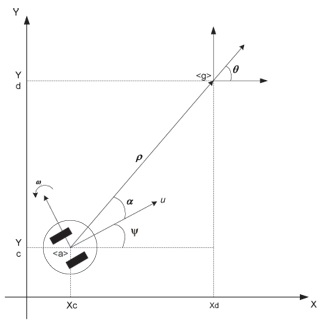
\includegraphics[scale=0.73]{./images/rob.jpg}
\captionof{figure}{\caption{Représentation Turtlebot}}
\end{figure}
Par la suite, nous prendrons deux vitesses de base, une linéaire et une angulaire, choisies en fonction du delta, de la moyenne, de la médiane et de la valeur de l'erreur de mesure. Le delta est l'écart entre la valeur minimale et maximale mesurées pour déterminer les valeurs aberrantes.\\
Si le delta est trop grand par rapport à la valeur moyenne, notre correction n'aura aucun effet puisque notre coefficient correcteur gardera cette incertitude de mesure.\\
En revanche, si la valeur moyenne est différente de la valeur médiane alors nous avons au moins une mesure aberrante.\\ 
Pour avoir un coefficient idéal, il faut un delta petit et une valeur moyenne sensiblement égale à la valeur médiane.\\


%Par la suite, nous prendrons deux vitesses de base, une linéaire et une angulaire, choisies en fonction du l'écart-type, de la moyenne, de la médiane et de la valeur de l'erreur de mesure. L'écart-type est nous permet de déterminer une tolérance pour les mesures.\\
%Si l'écart-type est trop grand par rapport à la valeur moyenne, notre correction n'aura aucun effet puisque notre coefficient correcteur gardera cette incertitude de mesure.\\
%En revanche, si la valeur moyenne est différente de la valeur médiane alors nous avons au moins une mesure aberrante.\\ 
%Pour avoir un coefficient idéal, il faut l'écart-type petit et la valeur moyenne sensiblement égale à la valeur médiane.\\


\section{Expérimentation}

\subsection{Ligne}

\subsubsection{Protocole}
Pour notre premier test de la ligne, nous avons pris des mesures en fonction de plusieurs vitesses et distances, 10 pour chaque cas.
Nous avons sélectionné les vitesses {0.1;0.5;0.7} $(m/s)$ pour couvrir notre correction. Nous avons choisi une vitesse lente pour éviter les dérapages et pour voir l'influence des forces de frottements, une vitesse médiane, et la vitesse maximale du robot. Pour les distances, nous avons pris {0.4;2.0} $m$.\\
Le protocole est le suivant:\\
\begin{itemize}
\item Programmer le robot pour un cas, avec les paramètres de vitesse et distance voulus. \\
\item Dessiner une ligne au sol et définir la position initiale.\\
\item Placer le robot au point de départ, puis relever les valeurs des ticks des roues droite et gauche, de la distance à $t_0$.\\
\item Lancer le programme, attendre la fin et relever les différentes valeurs avec le métre et le terminal.\\
\item Répéter le protocole 10 fois pour chacun des cas.\\
\end{itemize}
\vspace{5mm}

\begin{figure}[h]
    \begin{minipage}[c]{.46\linewidth}
        \centering
        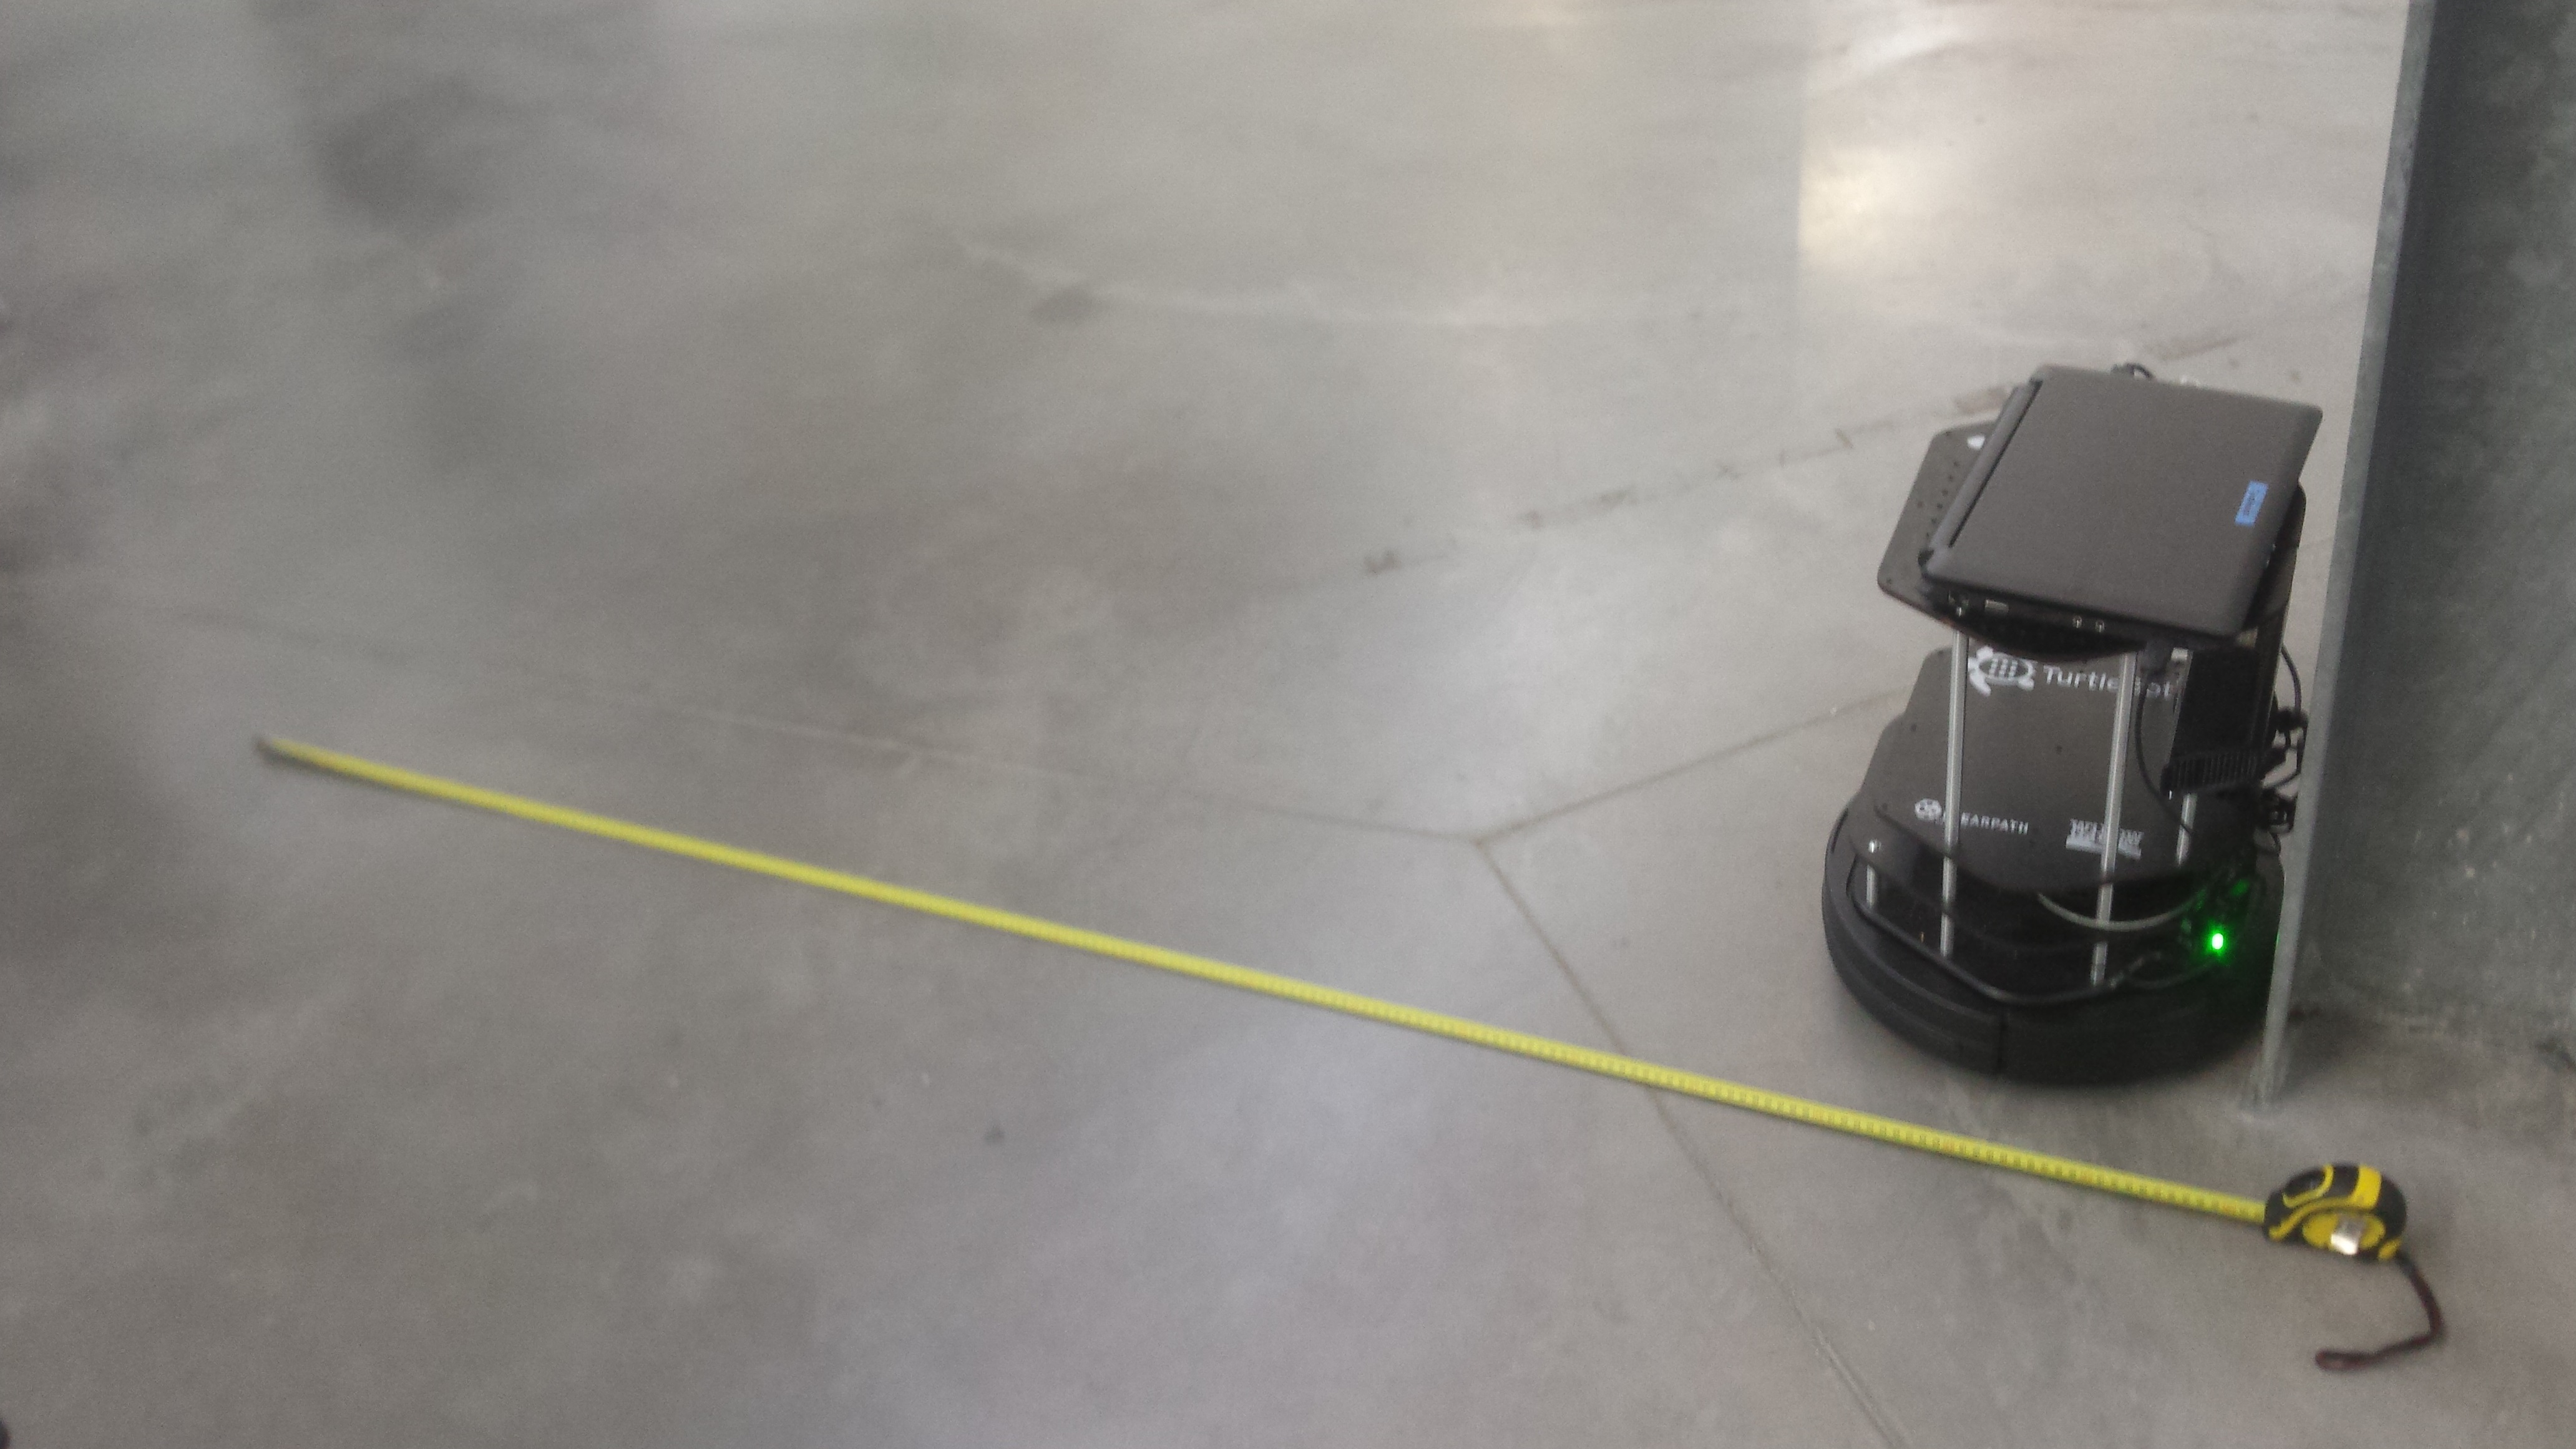
\includegraphics[width=1\textwidth]{./images/ml1.jpg}
        \captionof{figure}{\caption{Test ligne}}
    \end{minipage}
    \hfill%
    \begin{minipage}[c]{.46\linewidth}
        \centering
        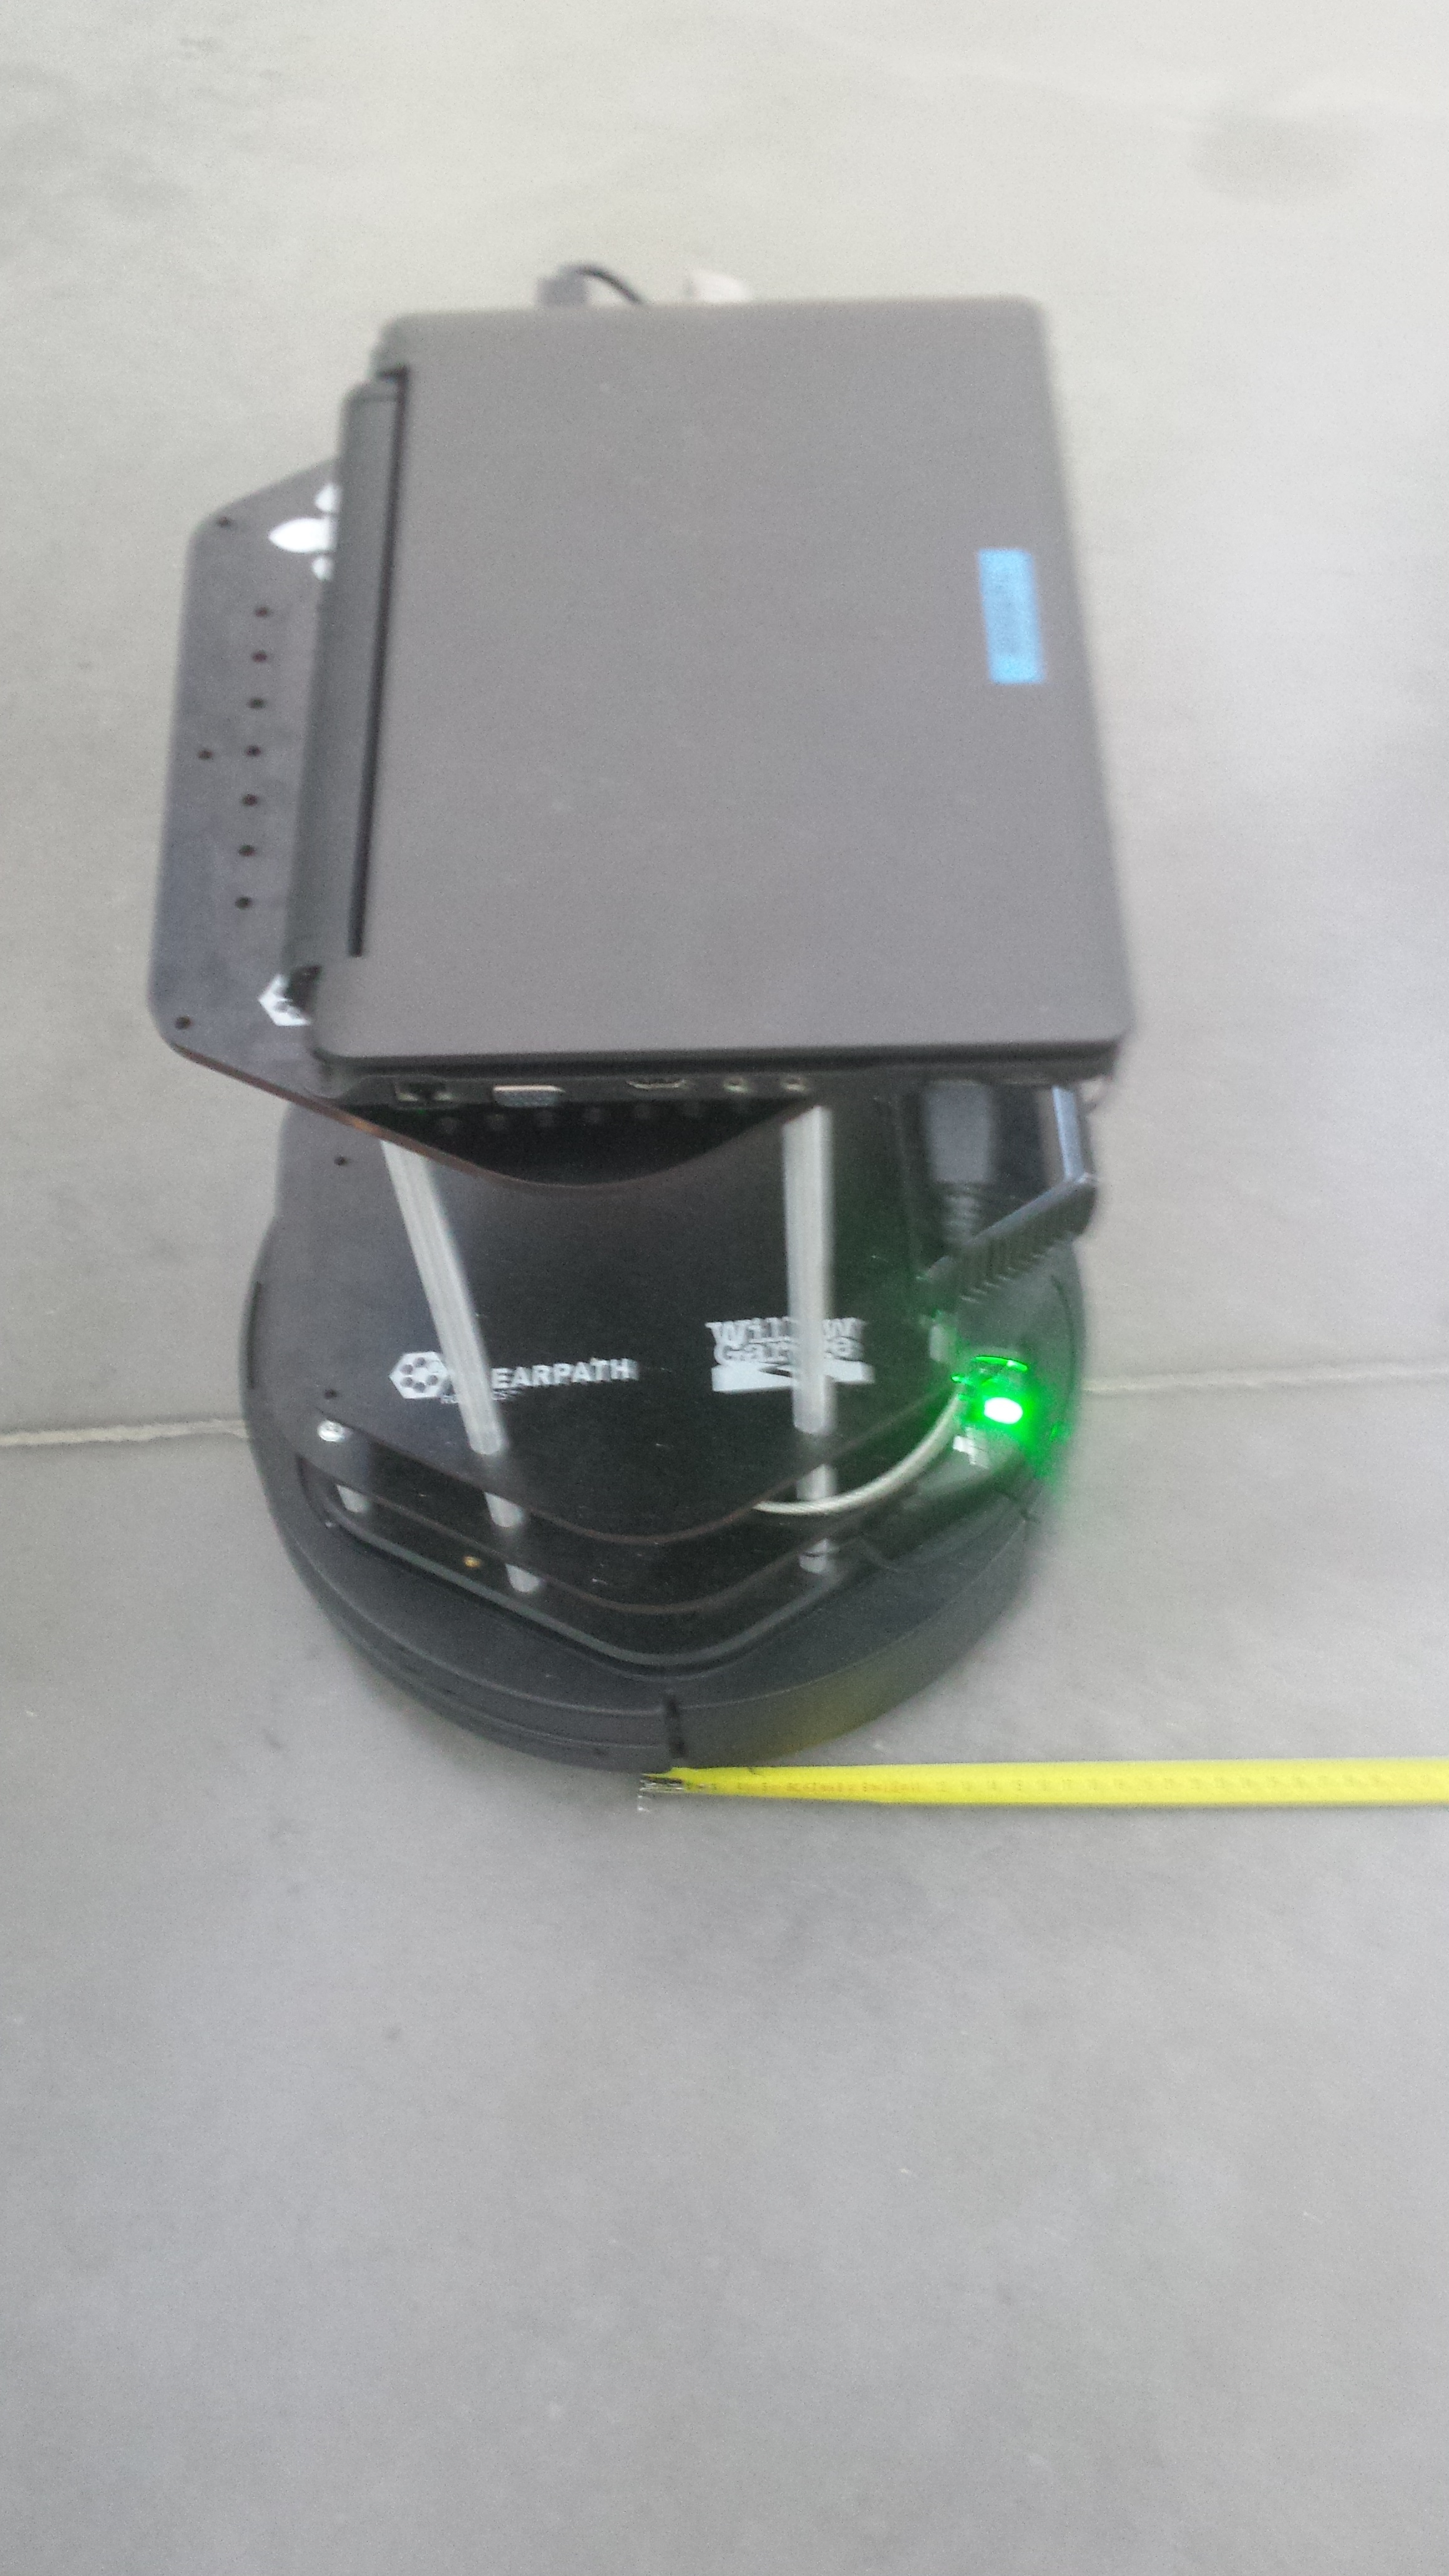
\includegraphics[width=0.35\textwidth]{./images/ml2.jpg}
        \captionof{figure}{\caption{Prise d'une mesure}}
    \end{minipage}
\end{figure}

\vspace{5mm}

\subsubsection{Résultats}

Sur les graphiques suivant, vous pouvez observer les résulats de nos mesures ainsi que l'erreur associée.\\

\vspace{5mm}

\begin{figure}[h]
\begin{minipage}{0.47\linewidth}
    	\centering
        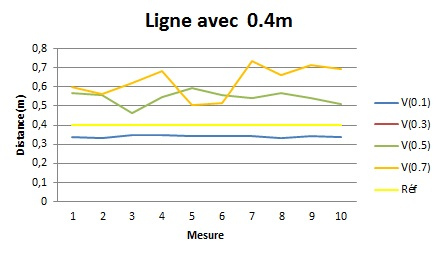
\includegraphics[scale=0.65]{./images/l0_4.jpg}
        \captionof{figure}{\caption{Courbes des distances parcourues pour 0,4 mètres en fonction des vitesses}}
    \end{minipage}\hfill
    \begin{minipage}[c]{.46\linewidth}
        \centering
        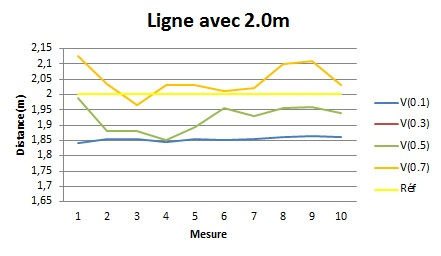
\includegraphics[scale=0.65]{./images/l2_0.jpg}
        \captionof{figure}{\caption{Courbes des distances parcourues pour 2,0 mètres en fonction des vitesses}}
    \end{minipage}
\end{figure}
\vspace{5mm}
\begin{figure}[h]
		\begin{minipage}{0.46\linewidth}
    	\centering
        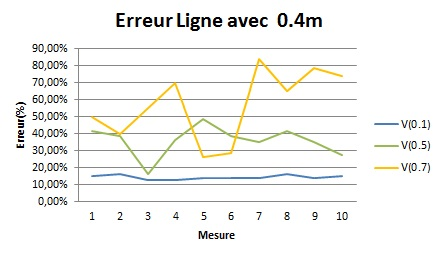
\includegraphics[scale=0.65]{./images/ErL0_4.jpg}
        \captionof{figure}{\caption{Courbes des erreurs pour 0,4 mètres en fonction des vitesses}}
    \end{minipage}\hfill
    \begin{minipage}[c]{.46\linewidth}
        \centering
        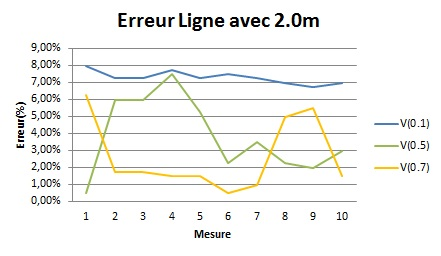
\includegraphics[scale=0.65]{./images/ErL2.jpg}
        \captionof{figure}{\caption{Courbes des erreurs pour 2,0 mètres en fonction des vitesses}}
    \end{minipage}
\end{figure}
\vspace{5mm}
\begin{figure}[h]
    \begin{minipage}[c]{.46\linewidth}
        \centering
        \begin{tabular}[c]{|l|c|c|r|}
 		\hline
  		Vitesse & 0.1 & 0.5 & 0.7 \\
  		\hline
  		Delta($\%$) & 3.75 & 32.50 & 57.50 \\
  		\hline
  		Delta($m$) & 0.015 & 0.13 & 0.23 \\
  		\hline
  		Moyenne($m$) & 0.340 & 0.54 & 0.63 \\
  		\hline
  		Médiane($m$) & 0.350 & 0.55 & 0.64  \\
  		\hline
		\end{tabular}
        \captionof{table}{\caption{Tableau comparatif pour la distance de 0,4 mètre}}
    \end{minipage}\hfill
    \begin{minipage}[c]{.46\linewidth}
        \centering
        \begin{tabular}[c]{|l|c|c|r|}
 		\hline
  		Vitesse & 0.1 & 0.5 & 0.7 \\
  		\hline
  		Delta($\%$) & 1.25 &7.00 & 5.75 \\
  		\hline
  		Delta($m$) & 0.025 & 0.14 & 0.16 \\
  		\hline
  		Moyenne($m$) & 1.854 & 1.926 & 2.046 \\
  		\hline
  		Médiane($m$) & 1.860 & 1.940 & 2.03  \\
  		\hline
		\end{tabular}
        \captionof{table}{\caption{Tableau comparatif pour la distance de 2,0 mètres}}
    \end{minipage}
\end{figure}

\vspace{5mm}

Nous remarquons que pour les vitesses basses, nous sommes toujours avec une valeur en dessous de celle attendue, tandis que pour la vitesse max nous sommes toujours au-dessus. La distance à parcourir est influencée par l'accélération et la décélération puisque nous ne les contrôlons pas, il en suit des dérapages. Ce qui induit une grande erreur pour les petites trajectoires.\\
Nous constatons que nous tournons autour de la valeur initiale de $11,7$ $tick/mm$ pour chacun des cas, même si pour certain nous avons une grosse erreur de distance. \\
Le delta des mesures est plus petit lorsque la vitesse est proche du minimal. Nous choisissons la vistesse qui à le delta le plus faible pour que notre correction soit efficace.\\
Les moyennes et médianes sont assez proches quelque soit la vitesse. \\


 

\subsubsection{Conclusion}

Pour améliorer la précision, il faudrait gérer l'accélération et la décélération dans le but d'avoir une trajetoire plus lisse.\\
Sur la courbe ci-dessous, nous avons le coefficient correcteur en fonction de la distance désirée.\\

\begin{figure}[!h]
    	\centering
        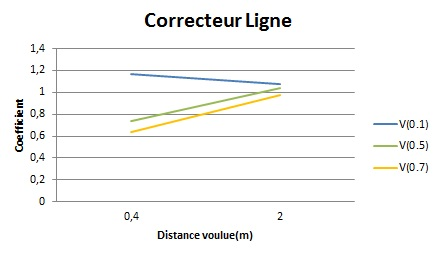
\includegraphics[scale=0.73]{./images/CRl.jpg}
        \captionof{figure}{\caption{Courbes des coefficients linéaires en fonction des vitesses}}
\end{figure}

Nous avons choisi de prendre la vitesse linéaire de 0,5 $m/s$.\\


\subsection{Rotation}

\subsubsection{Protocole}
Pour notre second test, la rotation, nous avons pris des mesures en fonction de plusieurs vitesses angulaires et angles, 10 pour chaque cas.
Les vitesses choisies sont {0.75;1.0;1.5;3.14} $(rad/s)$. Nous avons  du choisir cette vitesse angulaire minimale car le robot n'a pas de roues folles, il a des roues libres axées sur la translation. Par la suite, le choix de prendre deux valeurs intermédiaires nous a paru jusdicieux puisque le robot patine de temps en temps. Nous avons aussi pris la vitesse angulaire maximale du turtlebot puisque sa configuration initiale a une dégradation sur le gyroscope pour une vitesse supérieure à $1,92$ $radian/s$. Pour les distances, nous avons pris {pi/10;pi/4;pi} $radian$ étant donné qu'il fallait connaître la précision du robot pour des petites valeurs et un demi-tour.\\
Le protocole est le suivant:\\
\begin{itemize}
\item Programmer le robot pour un cas, avec les parmètres de vitesse angulaire et d'angle voulus.\\
\item Dessiner un cercle au sol ou un support troué et gradué, afin d'avoir la même surface, et définir la position initiale.\\
\item Placer le robot au point de départ, puis relever les valeurs des ticks des roues droite et gauche, d'orientation Z et W, de l'angle à $t_0$.\\
\item Lancer le programme, attendre la fin et relever les différentes valeurs avec le rapporteur et le terminal.\\
\item Répéter le protocole 10 fois pour chaque cas.\\
\end{itemize}
\vspace{5mm}

\begin{figure}[!h]
    \begin{minipage}[c]{.46\linewidth}
        \centering
        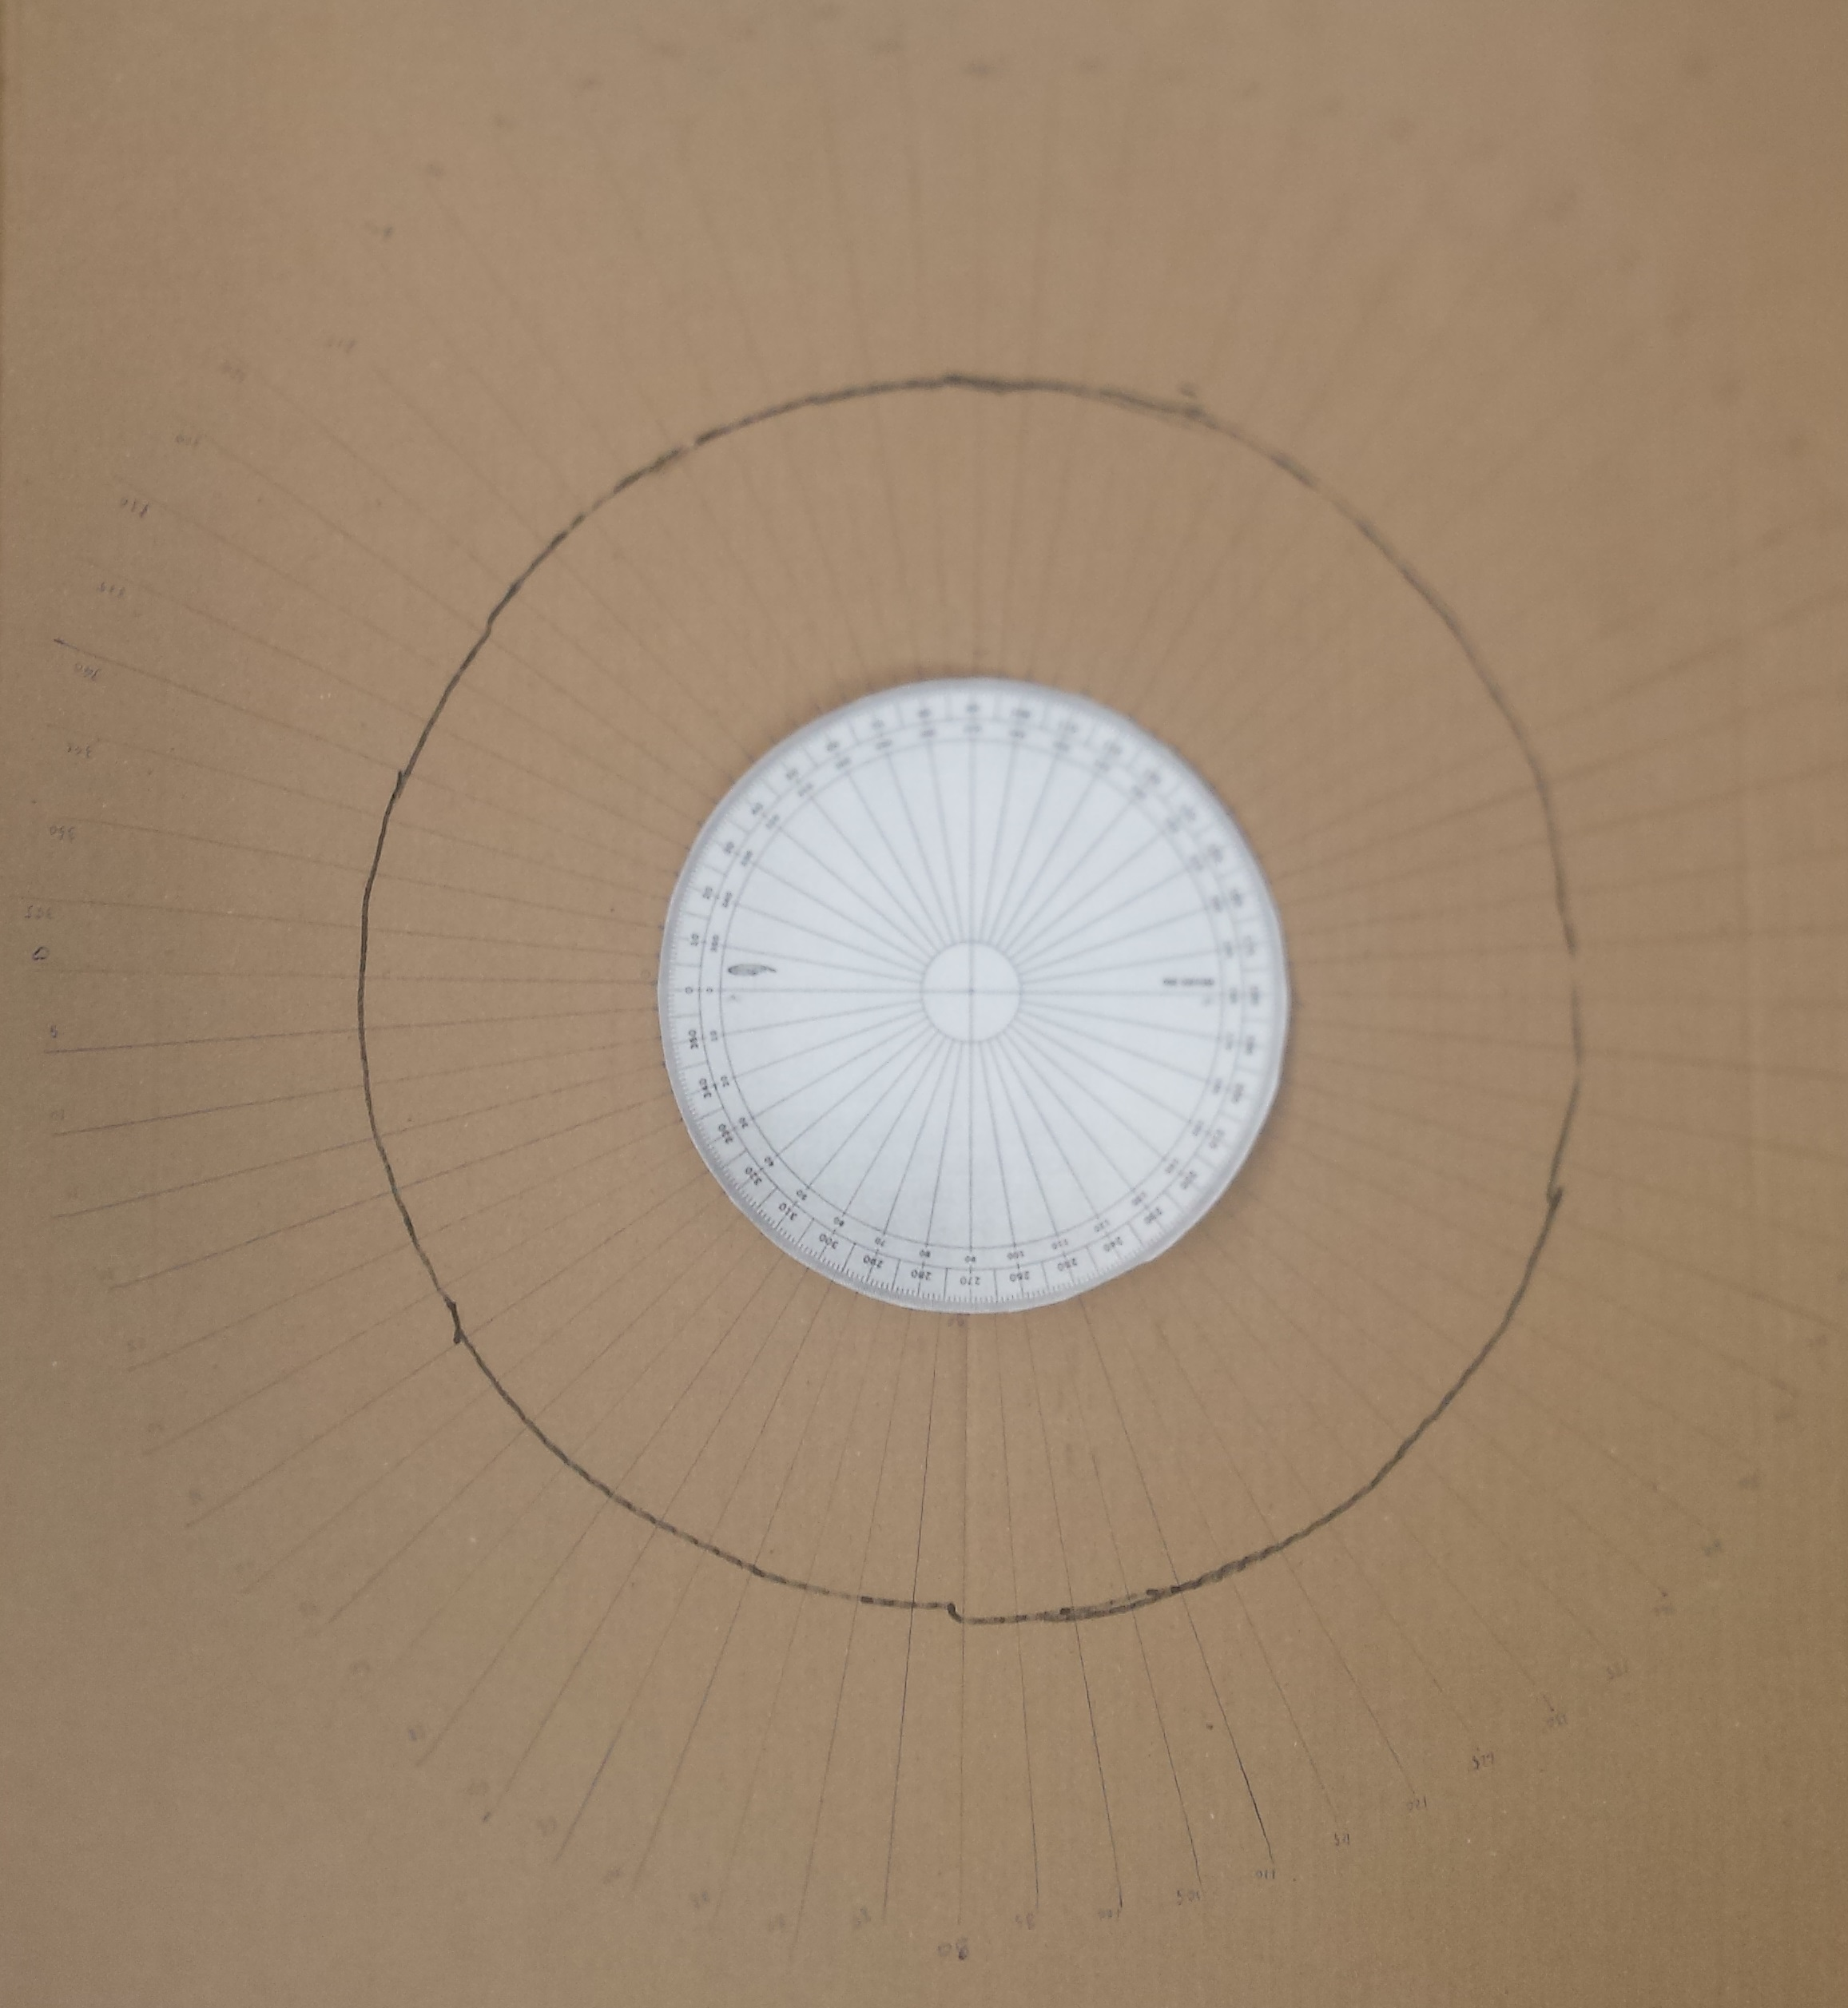
\includegraphics[scale=0.06]{./images/buildR.jpg}\tiny
        \caption{Rapporteur du turtlebot}
    \end{minipage}
    \hfill%
    \begin{minipage}[c]{.46\linewidth}
        \centering
        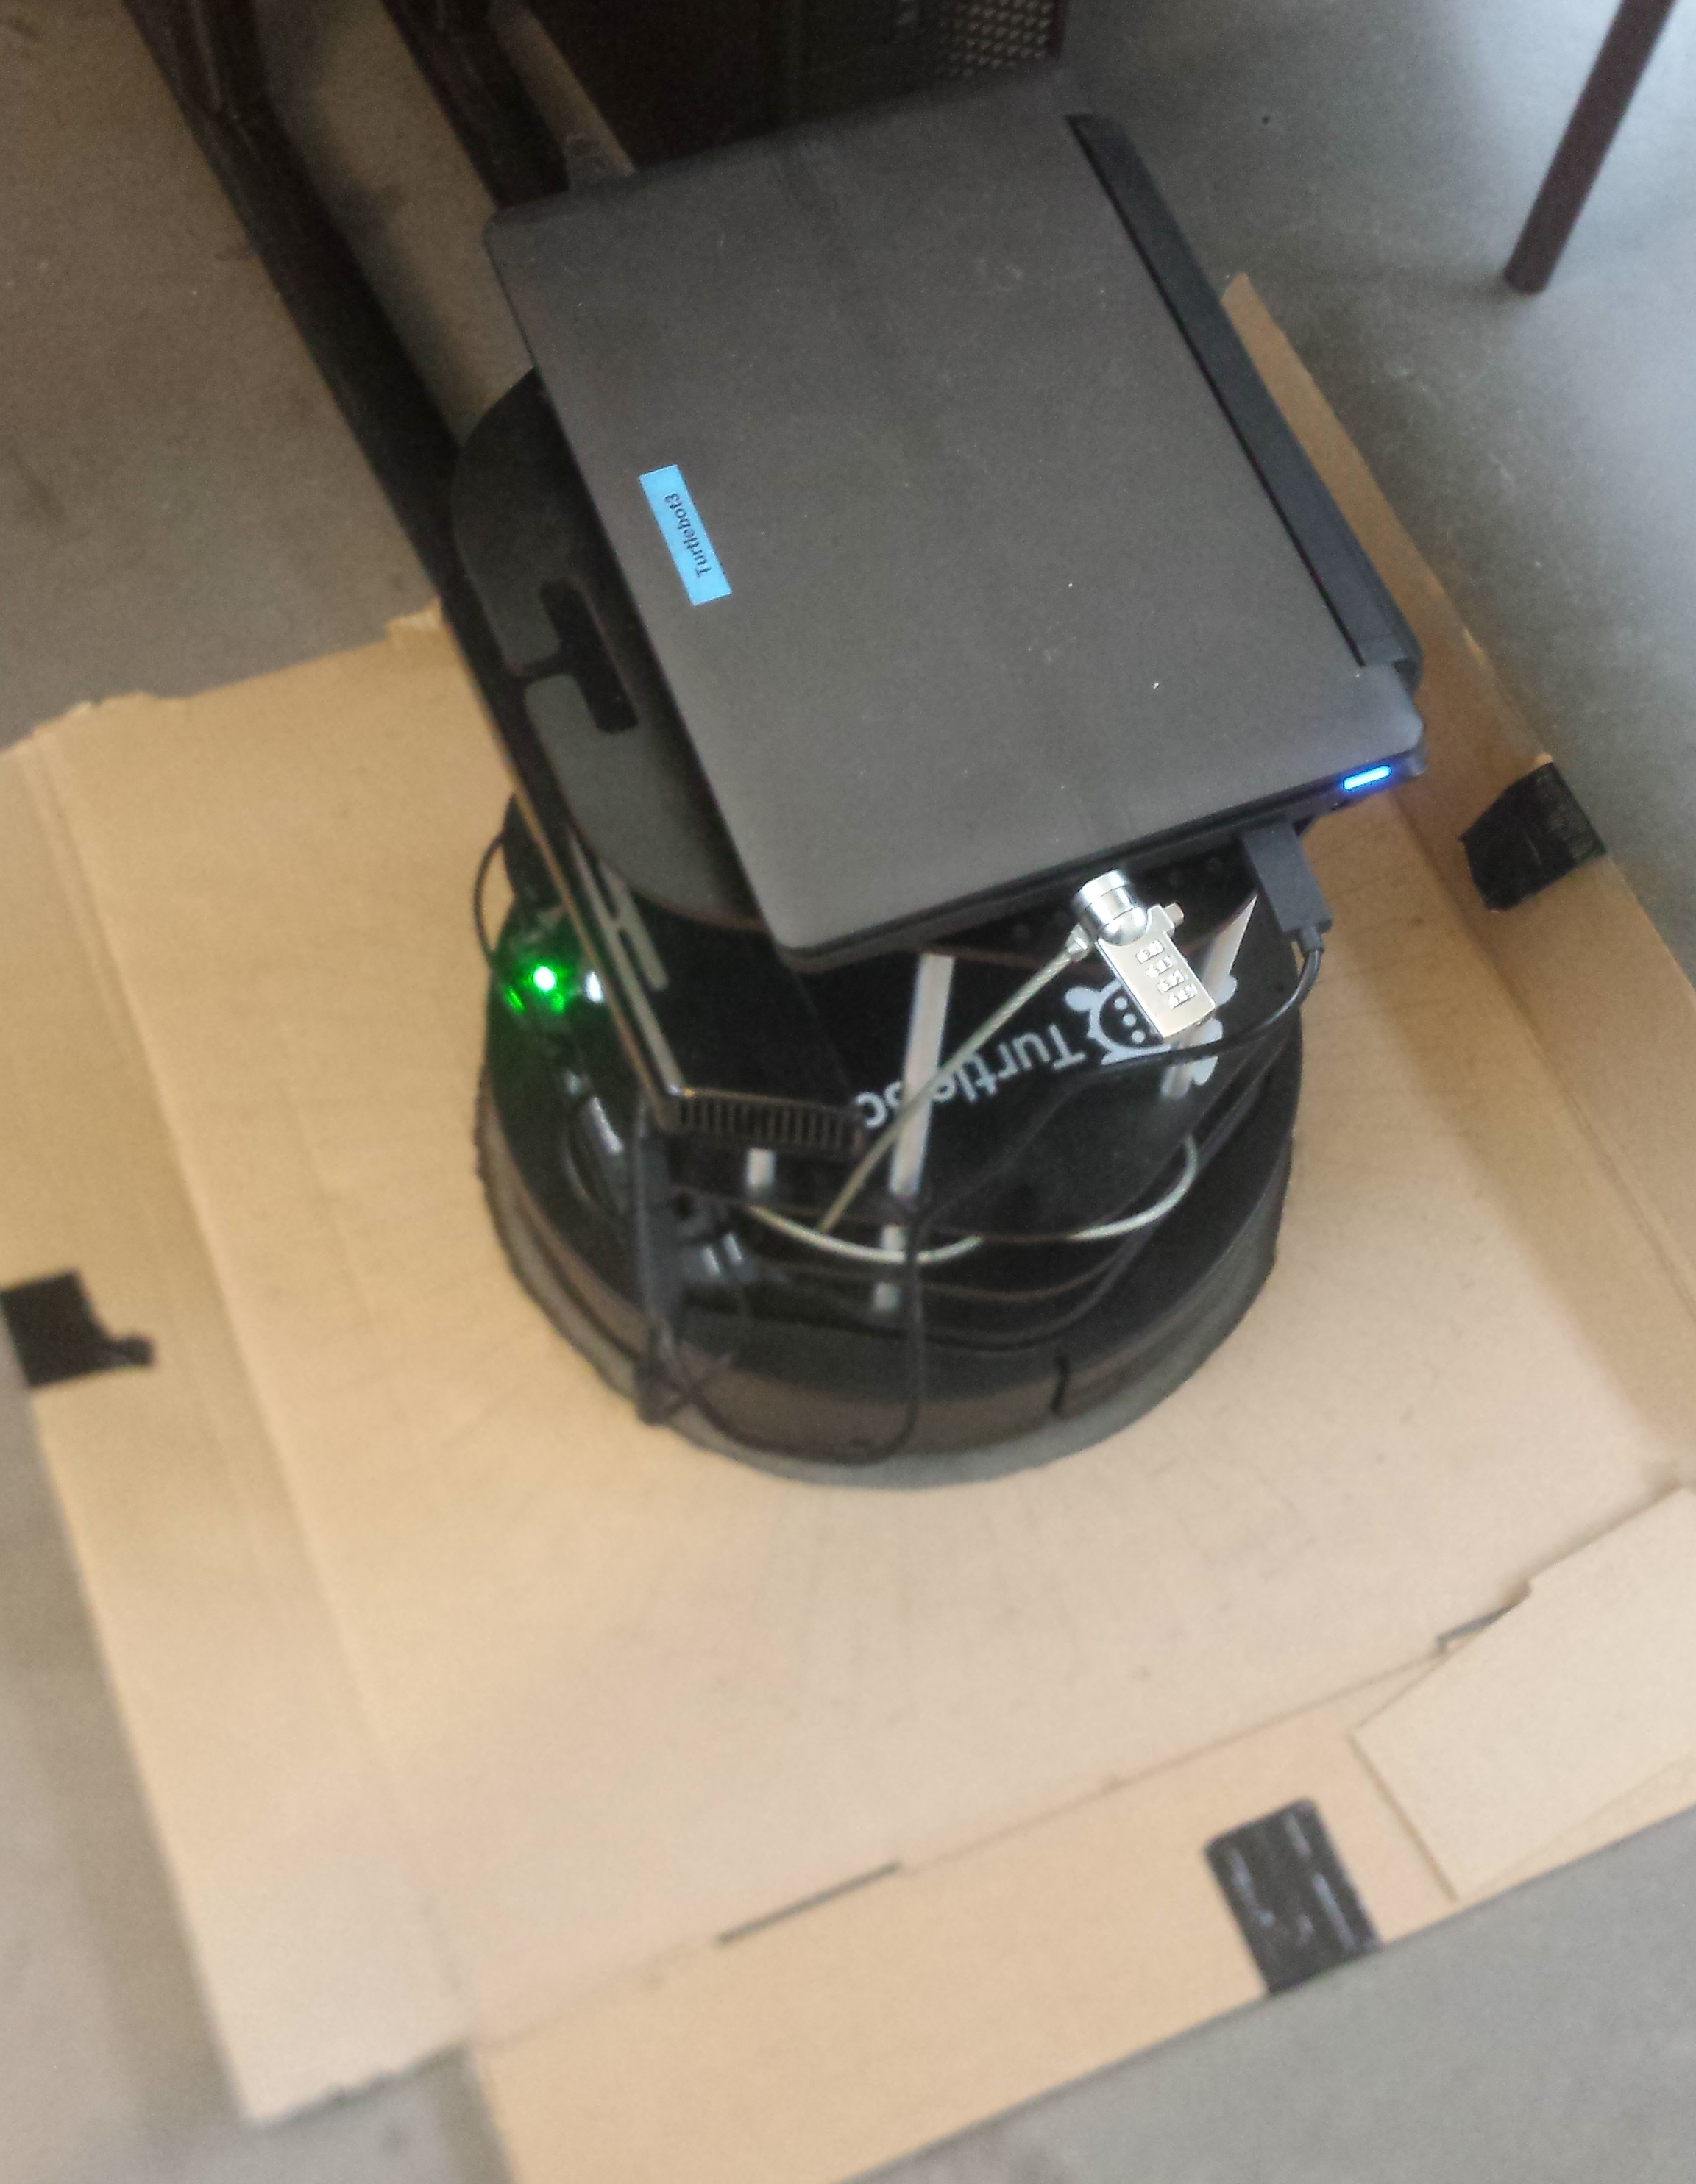
\includegraphics[scale=0.052]{./images/tr1.jpg}
        \caption{Prise d'une mesure}
    \end{minipage}
\end{figure}
\vspace{5mm}



\subsubsection{Résultats}

Lors de l'éxpérimentation, nous constatons que le turtlebot patine aléatoirement et qu'il faut une vitesse minimale pour dépasser la force de frottement exercée par les roues libres. \\

\vspace{5mm}
\begin{figure}[!]
\begin{minipage}{0.46\linewidth}
    	\centering
        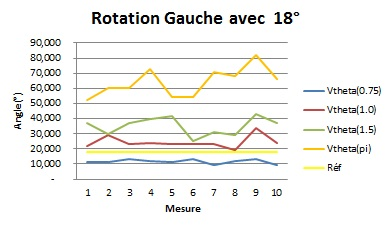
\includegraphics[scale=0.73]{./images/rg18.jpg}
        \captionof{figure}{\caption{Courbes des angles parcourus pour $pi/10$ radian en fonction des vitesses angulaires}}
    \end{minipage}\hfill
    \begin{minipage}[c]{.46\linewidth}
        \centering
        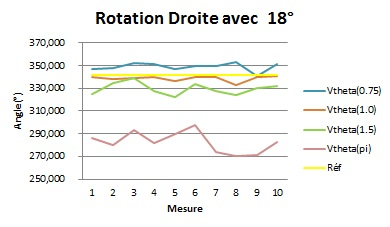
\includegraphics[scale=0.73]{./images/rd18.jpg}
        \captionof{figure}{\caption{Courbes des angles parcourus pour $-pi/10$ radian en fonction des vitesses angulaires}}
    \end{minipage}
\end{figure}

\begin{figure}[!]
    \begin{minipage}[c]{.46\linewidth}
        \centering
        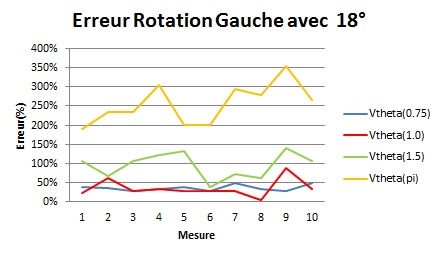
\includegraphics[scale=0.73]{./images/ErRg18.jpg}
         \captionof{figure}{\caption{Courbes des erreurs $pi/10$ radian en fonction des vitesses angulaires}}
    \end{minipage}
    \hfill%
    \begin{minipage}[c]{.46\linewidth}
        \centering
        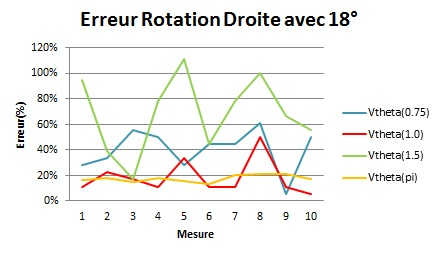
\includegraphics[scale=0.73]{./images/ErRd18.jpg}
        \captionof{figure}{\caption{Courbes des erreurs $-pi/10$ radian en fonction des vitesses angulaires}}
    \end{minipage}
\end{figure}

\begin{figure}[!]
    \begin{minipage}[c]{.46\linewidth}
        \centering
        \begin{tabular}{|l|c|c|c|r|}
 		\hline
  		Vitesse & 0.75 & 1 & 1.5 & pi \\
  		\hline
  		Delta($\%$) & 22.0 & 83.0 & 100.0 & 167.0 \\
  		\hline
  		Delta($rad$) & 0.07 & 0.262 & 0.314 & 0.524 \\
  		\hline
  		Moyenne($rad$) & 0.200 & 0.426 & 0.613 & 1.117 \\
  		\hline
  		Médiane($rad$) & 0.205 & 0.401 & 0.646 & 1.100 \\
  		\hline
		\end{tabular}
        \captionof{table}{\caption{Tableau comparatif pour l'angle de $pi/10$ radian}}
    \end{minipage}
    \hfill%
    \begin{minipage}[c]{.46\linewidth}
        \centering
        \begin{tabular}{|l|c|c|c|r|}
 		\hline
  		Vitesse & 0.75 & 1 & 1.5 & pi \\
  		\hline
  		Delta($\%$) & 56.0 & 44.0 & 94.0 & 8.0 \\
  		\hline
  		Delta($rad$) & 0.209 & 0.14 & 0.297 & 0.489 \\
  		\hline
  		Moyenne($rad$) & 0.192 & 0.372 & 0.529 & 1.349 \\
  		\hline
  		Médiane($rad$) & 0.175 & 0.349 & 0.541 & 1.353 \\
  		\hline
		\end{tabular}
        \captionof{table}{\caption{Tableau comparatif pour l'angle de $-pi/10$ radian}}
    \end{minipage}
\end{figure}

\begin{figure}[!]
\begin{minipage}{0.46\linewidth}
    	\centering
        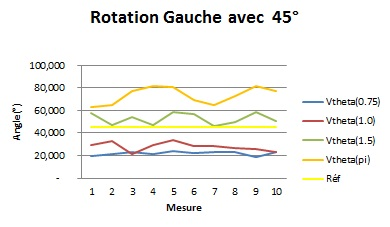
\includegraphics[scale=0.73]{./images/rg45.jpg}
        \captionof{figure}{\caption{Courbes des angles parcourus pour $pi/4$ radian en fonction des vitesses angulaires}}
    \end{minipage}\hfill
    \begin{minipage}[c]{.46\linewidth}
        \centering
        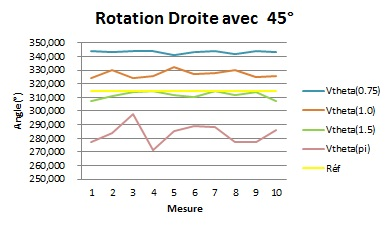
\includegraphics[scale=0.73]{./images/rd45.jpg}
        \captionof{figure}{\caption{Courbes des angles parcourus pour $-pi/4$ radian en fonction des vitesses angulaires}}
    \end{minipage}
\end{figure}
   
\begin{figure}[!]
    \begin{minipage}[c]{.46\linewidth}
        \centering
        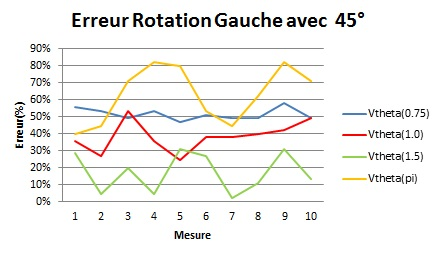
\includegraphics[scale=0.73]{./images/ErRg45.jpg}
        \captionof{figure}{\caption{Courbes des erreurs $pi/4$ radian en fonction des vitesses angulaires}}
    \end{minipage}
     \hfill%
    \begin{minipage}[c]{.46\linewidth}
        \centering
        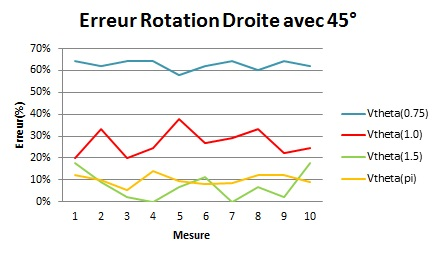
\includegraphics[scale=0.73]{./images/ErRd45.jpg}
        \captionof{figure}{\caption{Courbes des erreurs $-pi/4$ radian en fonction des vitesses angulaires}}
    \end{minipage}
\end{figure}

\begin{figure}[!]
    \begin{minipage}[c]{.46\linewidth}
        \centering
        \begin{tabular}{|l|c|c|c|r|}
 		\hline
  		Vitesse & 0.75 & 1 & 1.5 & pi \\
  		\hline
  		Delta($\%$) & 11.0 & 29.0 & 29.0 & 42.0 \\
  		\hline
  		Delta($rad$) & 0.087 & 0.227 & 0.227 & 0.332 \\
  		\hline
  		Moyenne($rad$) & 0.382 & 0.485 & 0.922 & 1.281 \\
  		\hline
  		Médiane($rad$) & 0.393 & 0.489 & 0.916 & 1.309 \\
  		\hline
		\end{tabular}
        \captionof{table}{\caption{Tableau comparatif pour l'angle de $pi/4$ radian}}
    \end{minipage}\hfill%
    \begin{minipage}[c]{.46\linewidth}
        \centering
        \begin{tabular}{|l|c|c|c|r|}
 		\hline
  		Vitesse & 0.75 & 1 & 1.5 & pi \\
  		\hline
  		Delta($\%$) & 7.0 & 18.0 & 18.0 & 9.0 \\
  		\hline
  		Delta($rad$) & 0.052 & 0.14 & 0.14 & 0.471 \\
  		\hline
  		Moyenne($rad$) & 0.293 & 0.572 & 0.843 & 1.340 \\
  		\hline
  		Médiane($rad$) & 0.218 & 0.480 & 0.707 & 1.396 \\
  		\hline
		\end{tabular}
        \captionof{table}{\caption{Tableau comparatif pour l'angle de $-pi/4$ radian}}
    \end{minipage}
\end{figure}

\begin{figure}[!]
\begin{minipage}{0.46\linewidth}
    	\centering
        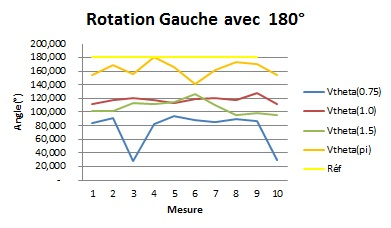
\includegraphics[scale=0.73]{./images/rg180.jpg}
        \captionof{figure}{\caption{Courbes des angles parcourus pour $pi$ radians en fonction des vitesses angulaires}}
    \end{minipage}\hfill
    \begin{minipage}[c]{.46\linewidth}
        \centering
        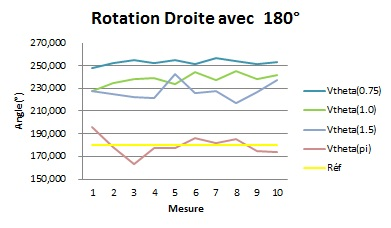
\includegraphics[scale=0.73]{./images/rd180.jpg}
        \captionof{figure}{\caption{Courbes des angles parcourus pour $-pi$ radians en fonction des vitesses angulaires}}
    \end{minipage}
\end{figure}

\begin{figure}[!]
    \begin{minipage}[c]{.46\linewidth}
        \centering
        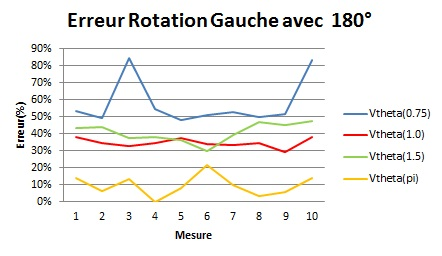
\includegraphics[scale=0.73]{./images/ErRg180.jpg}
        \captionof{figure}{\caption{Courbes des erreurs $pi$ radians en fonction des vitesses angulaires}}
    \end{minipage}
     \hfill%
    \begin{minipage}[c]{.46\linewidth}
        \centering
        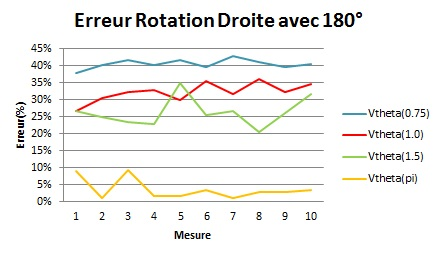
\includegraphics[scale=0.73]{./images/ErRd180.jpg}
        \captionof{figure}{\caption{Courbes des erreurs $-pi$ radians en fonction des vitesses angulaires}}
    \end{minipage}
\end{figure}

\begin{figure}[!]
    \begin{minipage}[c]{.46\linewidth}
        \centering
        \begin{tabular}{|l|c|c|c|r|}
 		\hline
  		Vitesse & 0.75 & 1 & 1.5 & pi \\
  		\hline
  		Delta($\%$) & 37.0 & 9.0 & 17.0 & 22.0 \\
  		\hline
  		Delta($rad$) & 1.152 & 0.279 & 0.541 & 0.681 \\
  		\hline
  		Moyenne($rad$) & 1.325 & 2.058 & 1.866 & 2.841 \\
  		\hline
  		Médiane($rad$) & 1.501 & 2.059 & 1.850 & 2.862 \\
  		\hline
		\end{tabular}
        \captionof{table}{\caption{Tableau comparatif pour l'angle de $pi$ radians}}
    \end{minipage}
    \hfill%
    \begin{minipage}[c]{.46\linewidth}
        \centering
        \begin{tabular}{|l|c|c|c|r|}
 		\hline
  		Vitesse & 0.75 & 1 & 1.5 & pi \\
  		\hline
  		Delta($\%$) & 5.0 & 9.0 & 14.0 & 8.0 \\
  		\hline
  		Delta($rad$) & 0.157 & 0.297 & 0.454 & 0.576 \\
  		\hline
  		Moyenne($rad$) & 1.871 & 2.129 & 2.314 & 3.154 \\
  		\hline
  		Médiane($rad$) & 1.876 & 2.129 & 2.330 & 3.185 \\
  		\hline
		\end{tabular}
        \captionof{table}{\caption{Tableau comparatif pour l'angle de $-pi$ radians}}
    \end{minipage}
\end{figure} 

\vspace{5mm}
A l'aide des graphiques, nous observons les variations des mesures par rapport à différente vitesse angulaire. Le robot a une meilleur précision lorsqu'il tourne dans le sens horaire.\\
Nous choisissons la vistesse qui à le delta le plus faible pour que notre correction soit efficace.\\
Le meilleur delta pour la rotation à gauche est à une vitesse angulaire de $0.75$ pour des angles inférieur à $pi/4$ $rad$ et de $1.0$ pour les angles supérieur à $pi/4$ $rad$. Celui pour la rotation à droite est à une vitesse angulaire de $0.75$ pour des angles supérieur à $pi/4$ $rad$ et de $pi$ pour les angles inférieur à $pi/4$ $rad$.\\
Les valeurs moyennes et médianes sont assez proches pour tous les cas, sauf pour la rotation à droite de $pi/4$ $radian$.\\

\vspace{5mm}
\subsubsection{Conclusion}

Pour avoir une meilleure précision dans notre rotation, il faudrait modifier les roues libres du turtlebot en roues folles dans le but de diminuer les forces de frottements exercés par ces dernières. \\
Sur la graphe ci-dessous, nous avons le coefficient correcteur en fonction de l'angle désiré pour les deux sens de rotations.\\


\vspace{5mm}
\begin{figure}[h]
\begin{minipage}{0.46\linewidth}
    	\centering
        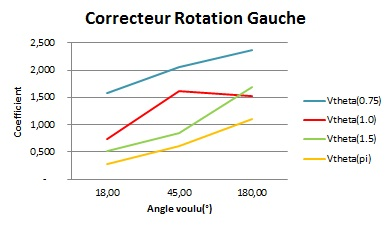
\includegraphics[scale=0.73]{./images/CRrg.jpg}
        \captionof{figure}{\caption{Courbes des coefficients pour la rotations à gauche en fonction des vitesses angulaires}}
    \end{minipage}\hfill
    \begin{minipage}[c]{.46\linewidth}
        \centering
        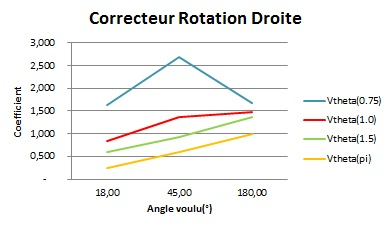
\includegraphics[scale=0.73]{./images/CRrd.jpg}
        \captionof{figure}{\caption{Courbes des coefficients pour la rotations à droite en fonction des vitesses angulaires}}
    \end{minipage}
\end{figure}
\vspace{5mm}

Nous avons choisi de prendre la vitesse angulaire de $0.75$ $rad/s$ pour la rotation à gauche et $1.5$ $rad/s$ pour la rotation à droite.\\


\section{Validation}

\subsubsection{Protocole}
Notre première étape étant faite, nous passons à la seconde pour vérifer nos coefficients linéaires et angulaires. Nous gardons le même procédé que précédement mais nous modifions notre distance désirée avec le correcteur adéquate et prenons l'erreur de mesure comme étant notre précision.\\
Nous partons du principe que nos coefficients sont juste.
Le protocole est le même que pour les premiers, à une différence près.\\
Pour la ligne : \\
\begin{itemize}
\item Programmer le robot pour un cas, avec les paramètres de vitesse et distance voulus. \\
\item Corriger l'angle avec le coefficient trouvé.\\
\item Placer le robot au point de départ, puis relever les valeurs des ticks des roues droite et gauche, de la distance à $t_0$.\\
\item Lancer le programme, attendre la fin et relever les différentes valeurs avec le métre et le terminal.\\
\item Répéter le protocole 10 fois pour chacun des cas.\\
\end{itemize}
\vspace{5mm}

Pour le cercle : \\
\begin{itemize}
\item Programmer le robot pour un cas, avec les parmètres de vitesse angulaire et d'angle voulus.\\
\item Corriger l'angle avec le coefficient trouvé.\\
\item Placer le robot au point de départ, puis relever les valeurs des ticks des roues droite et gauche, d'orientation Z et W, de l'angle à $t_0$.\\
\item Lancer le programme, attendre la fin et relever les différentes valeurs avec le rapporteur et le terminal.\\
\item Répéter le protocole 10 fois pour chaque cas.\\
\end{itemize}
\vspace{5mm}

%\\

Après plusieurs essais, il s'avère que certains coefficients sont faux. Et plus particulièrement, quand nous avons des petites distances ou angles. L'erreur peut venir de la précision de la mesure, du fait que le robot patine sur certaine rotation, ou encore du la latence du réseau.\\

\subsection{Choix des paramètres}
Pour conclure, ces expériences nous ont permis de trouver des vitesses idéales avec leur coefficient associés.
Nous avons choisis une vitesse linéaire de 0,5 $m/s$ et une vitesse angulaire de 1,5 $rad/s$.


\section{Conclusion}

Le rapport d'odométrie nous a permis d'avoir un déplacement plus précis pour notre navigation lors de notre première phase sur le Tp "Recherche Balle", de connaitre plus en détaille les caractéristiques et les noeuds utilisés par le turtlebot. Il faudrait refaire les tests en ajoutant les trajectoires cercle et  carré avec le robot modifié.\\
Même si par la suite nous avons utilisé une brique de l'environnement de ROS pour générer et suivre nos trajectoires. \\

\section{Code ROS}

\begin{DDbox}{\linewidth}
\begin{lstlisting}
#include "ros/ros.h"
#include "TurtleBotCommand.hpp"
#include "Odom.hpp"
#include "command.h"
#include "std_msgs/Bool.h"
#include <cmath>

#define FREQ 20 //10 Hz
#define pi 3.1415926535897932384626433832795

int main(int argc, char **argv)
{
    ROS_INFO("Launching odom_tests_node ...");
    ros::init(argc, argv, "odom_tests_node");
    ros::NodeHandle node;

    TurtleBotCommand turtleBot(node);
	Odom odom(node);

    ros::WallTime startTime;
    ros::WallDuration durationLine, durationAngle, durationWait(10);
    kobuki_msgs::SensorState tic;
    ros::Rate r(FREQ);

    int currentState = 0;
    bool start = false;
    float angularVelocity =0.1;
    float linearVelocity = 0.7;
    float angle = pi;
    float distance = 0.4;

    if (angularVelocity<0) durationAngle = ros::WallDuration(-angle/angularVelocity);
    else durationAngle = ros::WallDuration(angle/angularVelocity);

    if (linearVelocity<0) durationLine = ros::WallDuration(-distance/linearVelocity);
    else durationLine = ros::WallDuration(distance/linearVelocity);

    std::cout<<"angularVelocity : "<<angularVelocity<<std::endl;
    std::cout<<"linearVelocity : "<<linearVelocity<<std::endl;
    std::cout<<"angle : "<<angle<<std::endl;
    std::cout<<"distance : "<<distance<<std::endl;
    std::cout<<"durationAngle : "<<durationAngle<<std::endl;
    std::cout<<"durationLine : "<<durationLine<<std::endl;
\end{lstlisting}
\end{DDbox}
Suite Code : \\
\begin{DDbox}{\linewidth}
\begin{lstlisting}
    while(ros::ok())
	{
        ros::spinOnce();

	    //std::cout<<"currentState : "<<currentState<<std::endl;
	    switch (currentState)
        {
            case 0:
                if(!start)
                {
                    startTime = ros::WallTime::now();
                    start = true;
					ROS_INFO("Before Moving...");
					odom.displayMobileBaseSenorsCore();
					ROS_INFO("Moving...");
                }
                turtleBot.move(linearVelocity);
                if ((ros::WallTime::now() - startTime) > durationLine )
                {
                    currentState = 1;
                    start = false;
                }
                break;
            case 1:
                if(!start)
                {
                    startTime = ros::WallTime::now();
                    start = true;
					ROS_INFO("Before Turning...");
					odom.displayMobileBaseSenorsCore();
					ROS_INFO("Turning...");
                }
                turtleBot.turn(angularVelocity);
                if ((ros::WallTime::now() - startTime) > durationAngle)
                {
                    currentState = 0;
                    start = false;
                    ROS_INFO("Turning...");
                }
                break;
	    }
	    r.sleep();
	}
    return 0;
}
\end{lstlisting}
\end{DDbox}
\end{document}
%\begin{document}
% première page
\input{./Rapport_title.tex} 



%%%%%%%%%%%%%%%%%%%
% début du rapport
\newpage
\setcounter{page}{2}


\section{Introduction}


\begin{itemize}
\item Présentation du sujet
\item Nécessité du calibrage
\end{itemize}

\section{Définition}
\subsection{Odométrie}
L’odomètrie se définie comme la détermination d’un déplacement grâce à des odomètres. Ces derniers sont des capteurs embarqués qui mesurent une distance parcourue, les plus classiques sont des ensembles électromécaniques. Ils sont composés d’une roue en contact avec le sol et d’une roue dentée ou une roue codeuse entraînée par la première roue. Une paire de faisceaux lumineux (ou infrarouge) sera coupée (ou non) en fonction de la roue codeuse. L’ordre dans lequel les faisceaux sont coupés donne le sens de la rotation, le nombre de front donne le déplacement.
Il existe des capteurs magnétiques qui, au lieu d’entraîner une roue codeuse, font tourner un aimant. Un capteur fixe mesure l’orientation du champ magnétique et en déduit le déplacement.\\

\begin{itemize}
\item Qu'est-ce?
\item L'utilité
\item Laquelle utilisée
\end{itemize}

\subsection{Robot Holonome}
La détermination du mouvement (translation et rotation) d’un robot se fait généralement grâce à 2 odomètres.
Pour les robot holonomes, dont les roues peuvent aussi glisser sur le coté, nécessitent 3 odomètres.\\

\begin{itemize}
\item Qu'est-ce?
\item Notre robot
\end{itemize}

\section{Expérimentation}
Corriger les erreurs systématiques
\subsection{Principe}
\begin{itemize}
\item Modèle(choix trajectoire)
\item Développement modèle(choix des mesures)
\item Paramètres à trouver(linéaire et angulaire)
\item Détails des calculs 
\end{itemize}
\subsection{Résultats}
\begin{itemize}
\item Analyses(courbes, tableurs)
\item Conclusion(précision, erreurs, satisfaction)
\end{itemize}

\end{document}




Le « Cahier des Charges » est le suivant :
– Notre Arduino enverra toutes les 50/100ms, le nombres de tour de la roue droite et
gauche durant ces 50/100ms. Si on utilise plusieurs capteurs de distance, on enverra
également le numéros du capteur, ainsi que la distance de l’obstacle relevée à celui-ci.
– Le Pc devra à l’aide de ces préciseuses informations recalculer la position du robot
dans la pièce. Puis localiser l’obstacle dans cette même pièce.
– Une fois les positions du Robot et de l’obstacle connues, libre à vous de l’afficher à l’écran, la stocker sur la mémoire, l’envoyer par Wifi/Bluetooth…
Dans le programme java (NetBeans) que voici, la classe « Repertoire » est une des plus importantes.\\
Sa méthode « add(DistanceGauche, DistanceDroite, NumCapteur, Distance) » va recalculer la postion du Robot, ainsi que calculer la position de l’Obstacle, pour le mettre dans un Vector.\\

Recalculer la postion du robot\\
Quand il tourne à Gauche
Place aux mathématiques !
Le déplacement du robot sera relevé tout les 50/100ms, nous pouvons donc
considère que durant ce laps de temps la trajectoire du robot est un arc de cercle, avec
I comme centre instantané de rotation. À nous de déterminer le déplacement selon X, et Y, et la rotation selon Z.
beta : $angle RS^horizon$
alpha : angle que forme le robot et l’axe des abscisses
d-alpha : angle dut au déplacement du robot durant le mouvemet
dx : deplacement selon l’axe des X durant le mouvement
dy : déplacement selon l’axe des Y durant le mouvement
Le robot tournant à gauche, l’arc de la course de la roue Droite est plus grand que
celle de la roue Gauche. En vous aidant du dessin, vous remarquez que notre
déplacement se schématise à un triange IBC, avec AD parallèle à BC.
Dans cette situation Thalès nous dit : k = AD/BC = IA/IB.
Or rappelez vous, ce déplacement à lieu sur 50/100ms. Donc dans ces conditions,
nous pouvons considèrer que l’arc AD = segement AD, de même pour BC. Notre k
n’est donc plus une inconnue !
IA = k*IB= k*(IA+AB) = k*AB/(1-k)
PS : En toute logique AB = DC = ecart entre les roues.D’où IA est connue !
Toujours là ? alors on continue ! Dans le triangle AID et sa hauteur en I
$cos(A) = AD/(2*IA)$
$A = cos^-1((AD/(2*IA)$
$d-alpha = 180 -2*A$ Nous savons de combien notre robot à tourner durant le
mouvement !
Puis dans le triangle IRS et sa hauteur en I :
$OS = IS*sin(d-alpha/2)$
$RS = 2*(IA+AB/2)*sin(d-alpha/2)$
Voilà il ne manque plus qu’une chose pour finir calculer beta !
Les calculs de beta, dx, dy
Ces calculs n’ont rien de compliqué, mais ils changent tout le temps ! En
effet d’après le dessin et uniquement dans ce cas , nous avons
$beta = A-alpha$
$dx = -RS*cos(beta)$
$dy = -RS*sin(beta)$ (dy est négatif, car le repère est celui de l’écran !!!!!! )
Nous somme dans le cas où $alpha<A$ ! De même, si le robot contiue de tourner à
gauche, le signes de dy et dx changeront !
Alors comment faire ?
En voilà une bonne question ! à nous d’observer les changements pour disséquer les
cas. Ne sachant par où commencer, j’ai divisé mes obeservations en quatres parties :
0<alpha<90, 90<alpha<180, 180<alpha<270, 270<a<360… Originale !! Puis j’ai
répertorié les changements au sein des ces parties.\\

Voici le resultat :\\
Quand il tourne à Droite
Et oui, on recommence avec la Droite. Le calcule de d-alpha et RS sont quasiment
identique, il faut juste changer les segments utilisés, car maintenant c’est l’arc Gauche
qui est plus grand que l’arc Droit.
Une fois de plus ce qui est ennuyeux, c’est de disséquer chaque cas pour les calculs de
dx, dy, beta. Mais je vous ai donné la technique plus haut, donc au boulot !
Attention : J’ai pris le sens trigo, donc quand le robot tourne à Droite d-alpha est à
soustraire de alpha !
Pour ceux qui ont l’oeil, vous remarquerez le « – » dans le calcul de dy. Rappelez vous
! Les coordonnées sont par rapport au repère de l’écran.
Le plus dur est fait, nous savons désormais placer notre robot sur une carte en
fonction des ses tours de roues. Il ne manque plus qu’à localiser l’obstacle. Ensuite je
vous p

arlerais du fonctionnement général du programme.
Placer l’obstacle
En résumer, nous avons la position exacte du robot et son angle, la distance de
l’obstacle par rapport au robot, et le capteur utilisé.
Dans un premier temps, nous allons situer l’obstacle en prennant le robot comme
repère.
On notera (petit) x et (petit) y pour parler des ces coordonnées par rapport au robot.
x = Distance*cos(alpha+angleCapteur)
y = distance*sin(alpha+angleCapteur)
Mais nous voulons la position par rapport à l’écran, donc on convertit.
(grand) X et (grand) Y sont ces coordonnées par rapport à l’écran.\\